\title{Parametric RSA applied to Mixed-Gambles Task}
\author{Charles Zheng, Sanmi Koyejo and Russ Poldrack}
\date{\today}

\documentclass[12pt]{article} 

% packages with special commands
\usepackage{amssymb, amsmath}
\usepackage{epsfig}
\usepackage{array}
\usepackage{ifthen}
\usepackage{color}
\usepackage{fancyhdr}
\usepackage{graphicx}
\usepackage{mathtools}
\usepackage{csquotes}
\definecolor{grey}{rgb}{0.5,0.5,0.5}

\begin{document}
\maketitle

\newcommand{\tr}{\text{tr}}
\newcommand{\E}{\textbf{E}}
\newcommand{\diag}{\text{diag}}
\newcommand{\argmax}{\text{argmax}}
\newcommand{\Cov}{\text{Cov}}
\newcommand{\Var}{\text{Var}}
\newcommand{\argmin}{\text{argmin}}
\newcommand{\Vol}{\text{Vol}}
\newcommand{\comm}[1]{}

\newcommand{\bx}{\boldsymbol{x}}
\newcommand{\by}{\boldsymbol{y}}
\newcommand{\bX}{\boldsymbol{X}}
\newcommand{\bY}{\boldsymbol{Y}}


\section{Introduction}

\section{Data}

We used the mixed-gambles data from Tom et al. 2007.
The data consisted of 3 runs for each of 16 subjects.
In each run, 16 different gambling tasks were presented.
These tasks varied in the gain amount and loss amount.

Clusters were obtained using a parametric map from {\tt http://neurovault.org/images/10680/},
then applying thresholding using FSL.
A size threshold was applied, yielding 28 regions of interest.

\begin{figure}[h]
\centering
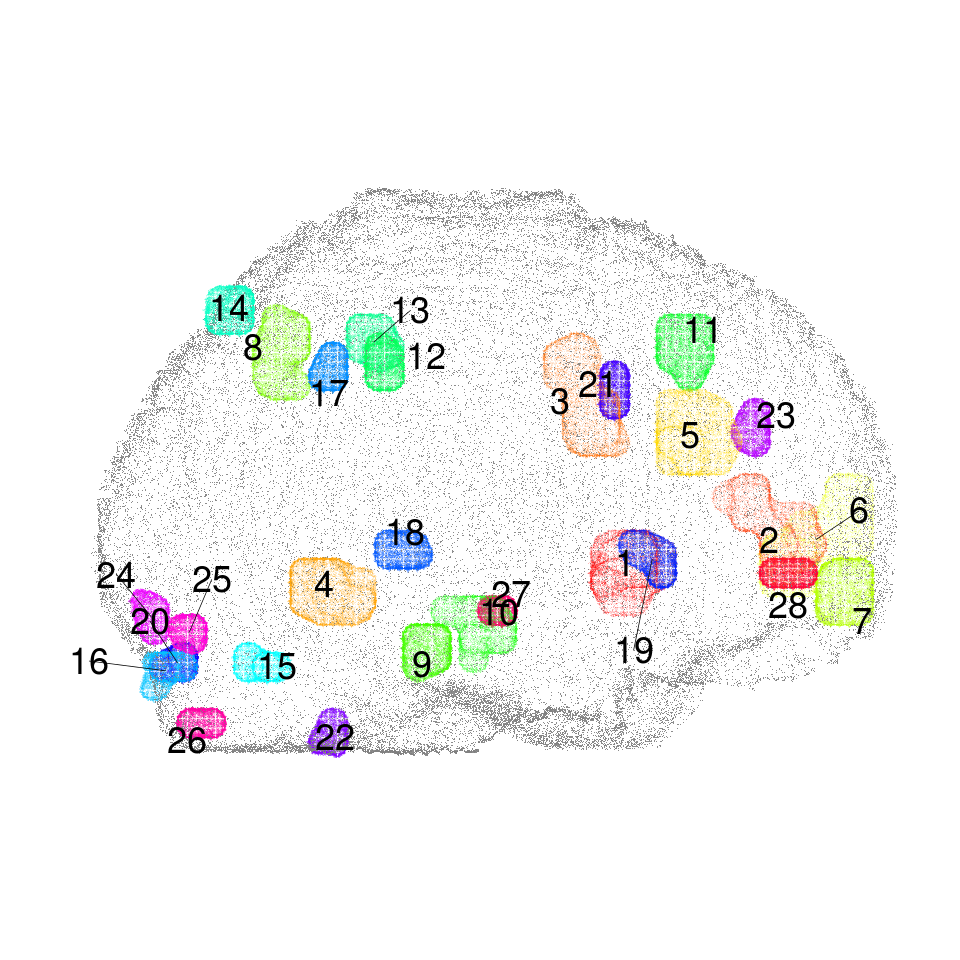
\includegraphics[scale = 0.1]{../a7plots/all_rois_view1.png}
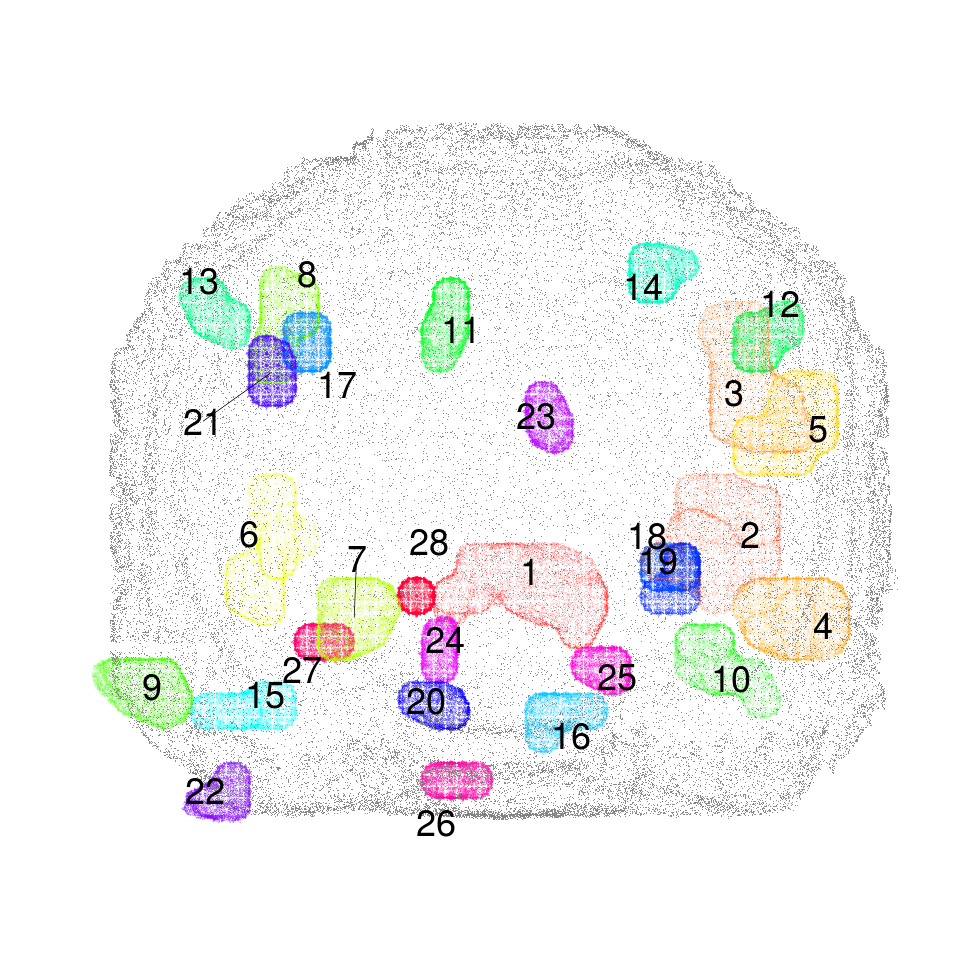
\includegraphics[scale = 0.1]{../a7plots/all_rois_view2.png}
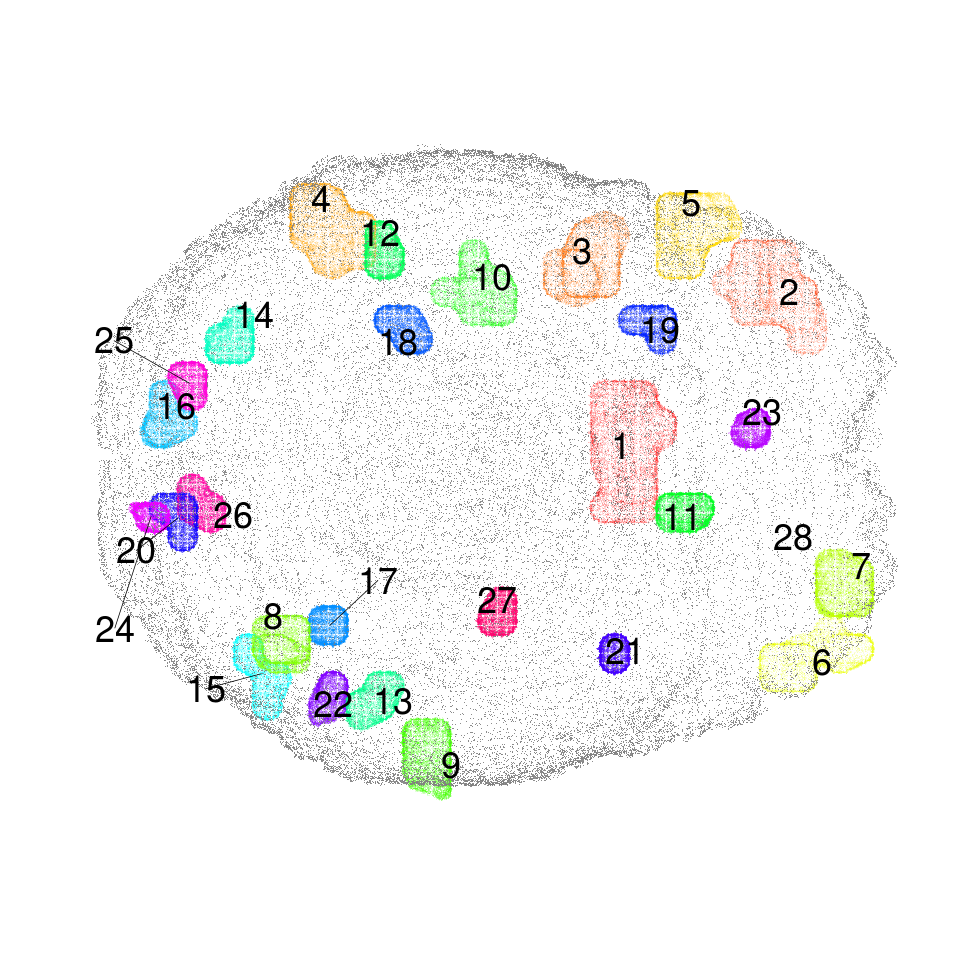
\includegraphics[scale = 0.1]{../a7plots/all_rois_view3.png}
\caption{Regions of interest.}
\end{figure}

The scans were registered to a common template, then a standard linear model-based approach
was used to extract an activity level per voxel per event per run.
We extracted the regions of interest from the data.  For a given region of interest, the data takes the form:

\begin{tabular}{|c|c|c|c||c|c|c|c|}
\hline
subject & run & gain & loss & voxel 1 & voxel 2 & ... & voxel $N$ \\
\hline
 1 & 1 & 13 &  6.5 & -222.8994 &  -373.85025 & ... & 12.038\\
... & ... & ... & ... & ... & ... & ... & ...\\
16 & 3 & 37 & 18.5 & -136.89 & -73.49 & ... & 75.068146 \\
\hline
\end{tabular}

where $N$ is the number of voxels in the ROI.


\end{document}



